\documentclass{report}

\usepackage{german}
\usepackage[T1]{fontenc}
\usepackage[utf8]{inputenc}
\usepackage{tikz}
\usepackage{pgfplots}
\usepackage{custompkg}

\begin{document}
	
	\bslinespacing{1.5}
	
	\begin{itemize}
		\item Der Wien-Filter kann verschiedene Massen aussortieren.
	\end{itemize}
	
	
	\begin{table}[h]		
		\begin{tabular}{|c|c|c|c|c|c|c|}
			\hline
			\textbf{I/A} & 0 & 2 & 4 & 6 & 8 & 10.5 \\
			\hline
			\textbf{$m/g$} & 0 & 2.1 & 3.2 & 5.2 & 6.5 & 8.6 \\
			\hline
			\textbf{$\frac{F_G = F_L}{mN}$} & 0 & 21 & 32 & 52 & 65 & 86 \\
			\hline
		\end{tabular}
	\end{table}
	
	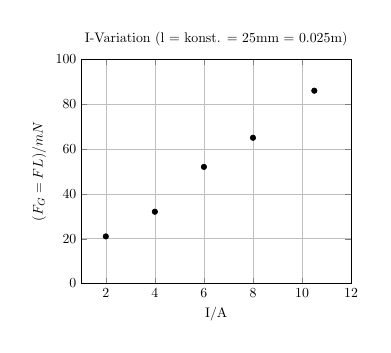
\begin{tikzpicture}[scale=0.5]
		\begin{axis}
			[
				title={I-Variation (l = konst. = 25mm = 0.025m)},
              xlabel={I/A},
              ylabel={$(F_G = FL) / mN$},
              grid,
              xmin=1,
              xmax=12,
              ymin=0,
              ymax=100
            ]
            \addplot [only marks] table {
					2 21
					4 32
					6 52
					8 65
					10.5 86
			  };
        \end{axis}
    \end{tikzpicture}

	\newpage
	
		\begin{table}[h]		
		\begin{tabular}{|c|c|c|c|c|}
			\hline
			\textbf{l/m} & 0 & 0.0125 & 0.025 & 0.1 \\
			\hline
			\textbf{$m/g$} & 0 & 3.3 & 6 & 19.5 \\
			\hline
			\textbf{$\frac{F_G = F_L}{mN}$} & 0 & 33 & 60 & 195 \\
			\hline
		\end{tabular}
	\end{table}
	
	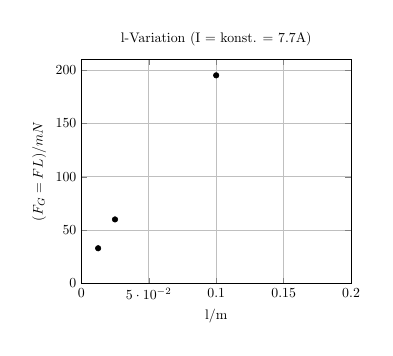
\begin{tikzpicture}[scale=0.5]
		\begin{axis}
			[
				title={l-Variation (I = konst. = 7.7A)},
              xlabel={l/m},
              ylabel={$(F_G = FL) / mN$},
              grid,
              xmin=0,
              xmax=0.2,
              ymin=0,
              ymax=210
            ]
            \addplot [only marks] table {
                	0.0125 33
					0.025 60
					0.1 195
			  };
        \end{axis}
    \end{tikzpicture}

	\begin{table}[h]		
		\begin{tabular}{ccccccc}
			$F_L =$ & I $\times$ & L $\times$ & B = & e & $\times \frac{l}{t}$ & $\times B$ \\
			 & (Stromstärke  & & & & Weg, den das Elektron & \\
			 & = $\frac{Ladung}{Zeit}$) & & & & in einer Zeit zurücklegt & \\
			 \hline
			 = e $\times$ & v $\times$ & B & & 
		\end{tabular}
	\end{table}
	
	\begin{table}[h]
		\begin{tabular}{ccccccccc}
			1) & $r=5cm=$ & $m$; & $B=1,12mT=$ & T; & $U_B=240V$ & $\to$ & $m_e=$ \\
			2) & $r=4cm=$ & $m$; & $B=1,5mT=$ & T; & $U_B=300V$ & $\to$ & $m_e=$ \\
			3) & $r=3cm=$ & $m$; & $B=2,175mT=$ & T; & $U_B=360V$ & $\to$ & $m_e=$ \\
			4) & $r=3cm=$ & $m$; & $B=2,375mT=$ & T; & $U_B=400V$ & $\to$ & $m_e=$ \\
		\end{tabular}
	\end{table}
	\newpage
	\begin{table}[h]
		\begin{tabular}{cccc}
			Lorentz: &$F_L = I \times l \times B$ & bzw. & $F_L = e \times v \times B$ \\
			&(kompletter Draht) & & (einzelnes Elektron) \\
			Elektrisch: &$F_E = E \times Q = \frac{U}{d} \times Q$ & bzw. & (siehe 1.3) \\
			siehe Beschreibung & $F_L = F_E$ & $\Leftrightarrow$ & $e \times v \times B = \frac{U}{d} \times e$ \\
		\end{tabular}
	\end{table}
	
	\newpage
	
	\begin{table}[h]
		\begin{tabular}{cc}
			$v = \frac{E}{B} = \frac{U_K}{B \times d}$ & \\
			aus 1.7: & $F_E = F_L$ \\
			& $v = \frac{U}{v \times d}$ \\
			& $v = \frac{U}{B \times d}$ \\
		\end{tabular}
	\end{table}
	
	
\end{document}